\documentclass{letter}
\usepackage{amsmath, amsthm, amssymb, graphicx, enumitem, esvect}
\graphicspath{ {./images/} }

% Language setting
% Replace `english' with e.g. `spanish' to change the document language
\usepackage[english]{babel}

% Set page size and margins
% Replace `letterpaper' with `a4paper' for UK/EU standard size
\usepackage[letterpaper,top=0.1cm,bottom=0.2cm,left=0.2cm,right=0.2cm,marginparwidth=0cm]{geometry}

\begin{document}
\textbf{Monotone Convergence Theorem:} Monotone inc/dec and bounded
above/below $\implies (x_n)$ converges. \\
\textbf{Bolzono-Weirstrauss Theorem:} Bounded $\implies \exists
(x_{n_k})$ that converges. \\
\textbf{Squeeze Theorem:} Given $(x_n), \ (y_n), \ (z_n) : y_n \leq
x_n \leq z_n \forall n \in \mathbb{N}$ and $y_n \to x, \ z_n \to x$ as
$n \to \infty$, $x_n \to x$ as $n \to \infty$. \\
\textbf{Test for Divergence:} $(x_n) \not\rightarrow 0 \implies \sum x_n$ does
not converge. \\
\textbf{Cauchy Sequence:} $\forall \varepsilon > 0, \exists N \in
\mathbb{N} : \forall n,m > N, |x_n - x_m| <
\varepsilon$. \textit{\textbf{Note:}} $(x_n)$ is cauchy $\iff (x_n)$
converges in $\mathbb{R}$ only. \\
\textbf{Geometric Series:} Given $x \in \mathbb{R}$, $S_n =
\sum\limits_{k = 1}^{n} x^k = \frac{1 - x^{n + 1}}{1 - x}$ if $x \neq
1$. $|x| < 1 \implies S_n \rightarrow \frac{1}{1 - x} \implies (x)^n
\rightarrow 0$ by ALT. $|x| > 1 \implies S_n \rightarrow +\infty$. \\
\textbf{Comparison Test:} Assume $y_n \geq 0 \ \forall n \geq
N$. If $|x_n| \leq y_n \forall n \in \mathbb{N}$, then: \\
(i) $\sum y_n$ converges $\implies \sum x_n$ converges. \\
(ii) $\sum |x_n|$ diverges $\implies \sum y_n$ diverges. \\
(iii) $\sum y_n \rightarrow +\infty \ \& \ x_n \geq y_n, \forall n \in
\mathbb{N} \implies \sum x_n \rightarrow +\infty$. \\
\textbf{Absolute Convergence Test:} $\sum |x_n|$ converges $\implies
\sum x_n$ converges. \\
\textbf{Cauchy Condensation Test:} Given $(x_n)$ decreasing and
nonnegative, $\sum\limits_{n = 1}^{\infty} x_n$ converges $\iff
\sum\limits_{n = 1}^{\infty} 2^nx_{2^n}$ converges. \\
\textbf{Cauchy Criterion:} $\sum\limits_{n = 1}^{\infty} x_n$
converges $\iff \forall \varepsilon > 0, \exists N \in \mathbb{N} : n
> m \geq N \implies |x_{m + 1} + \cdots + x_n| < \varepsilon$. \\
\textbf{p-series Test:} $\sum\limits_{n = 1}^{\infty} \frac{1}{n^p}$
converges $\iff$ $p > 1$. \\
\textbf{Ratio Test:} Given $x_n \neq 0$, $\lim\limits_{n \to
  \infty}\left| \frac{x_{n + 1}}{x_n} \right| = L$ converges absolutely
if $L < 1$, diverges if $L > 1$, inconclusive if $L = 1$. \\
\textbf{Root Test:} Given $x_n$, $\lim\limits_{n \to \infty}
\left|x_n\right|^{\frac{1}{n}} = L$ converges absolutely if $L < 1$, diverges if
  $L > 1$, inconclusive if $L = 1$. \\
\textbf{Alternating Series Test:} If a sequence $(x_n)$ is decreasing
and converges to 0, then $\sum (-1)^{n + 1} x_n$ converges. \\
\textbf{Exponent rules with $e$:} $x^a = e^{a \log x}$ \\
\textbf{Existance of Limits:} $\lim\limits_{x \to c} f(x)$ exists
$\iff \lim\limits_{x \to c^-} f(x) = \lim\limits_{x \to c^+} f(x)$ \\
\textbf{Continuity ($\varepsilon, \delta$):} $f: A \to \mathbb{R}$ is
continuous at $c \in A$ if $\forall \varepsilon > 0, \exists \delta >
0$ s.t. whenever $x \in A, |x - c| < \delta$, we have $f(x) - f(c)| <
\varepsilon$. \\
\textbf{Functional Limit ($\varepsilon, \delta$):} $\lim\limits_{x \to
  c} f(x) = L \iff $ for $c \in L_A$ if $\forall \varepsilon > 0,
\exists \delta > 0$ s.t. whenever $x \in A, 0 < |x - c| < \delta$, we
have $f(x) - L| < \varepsilon$. \\ \\
\textbf{Prove using the ($\varepsilon, \delta$) definition that $f(x) =
\sqrt{x + \sqrt{x}}$ is continuous on $[0, +\infty)$.} \\
\textit{\textbf{Scratch:}} Case 1: $c = 0$. Then, $|f(x) - f(0)| =
\sqrt{x + \sqrt{x}} \leq \sqrt{2\sqrt{x}} =
2^{\frac{1}{x}}x^{\frac{1}{4}}$. $x < \delta \implies \delta \leq
\frac{1}{4}\varepsilon^4$. \\
\textit{\textbf{Proof:}} Let $\varepsilon > 0$. Choose $\delta =
\min{\left\{1, \frac{1}{4}\varepsilon^4\right\}}$. Then, $|f(x) - f(0)| =
\sqrt{x + \sqrt{x}} \leq \sqrt{2\sqrt{x}} =
2^{\frac{1}{x}}x^{\frac{1}{4}} < \varepsilon$ whenever $0 \leq x <
\delta$. \\
\textit{\textbf{Scratch}} Case 2: $c \neq 0$. Then, we have:
\begin{align*}
  0 < |f(x) - f(c)|
  &= \left|\sqrt{x + \sqrt{x}} - \sqrt{c + \sqrt{c}}\right| \\
  &= \frac{|x + \sqrt{x} - c - \sqrt{c}|}{|\sqrt{x + \sqrt{x}} + \sqrt{c + \sqrt{c}}|}
    \leq \frac{|x  - c + \sqrt{x} - \sqrt{c}|}{|\sqrt{c + \sqrt{c}}|} \\
  &= \frac{|x - c + \frac{x - c}{\sqrt{x} + \sqrt{c}}|}{|\sqrt{c + \sqrt{c}}|}
     \leq \frac{\left|x - c\right| + \left|\frac{x - c}{\sqrt{c}}\right|}{|\sqrt{c + \sqrt{c}}|} \\
  &= \frac{\left(|x - c|\right)\left(\sqrt{c} + 1\right)}{\sqrt{c}\sqrt{c + \sqrt{c}}} < \varepsilon \\
  &\implies \delta = \frac{\sqrt{c}\sqrt{c + \sqrt{c}}}{\sqrt{c} + 1}\varepsilon 
\end{align*}
\textit{\textbf{Proof:}} Let $\varepsilon > 0$. Choose $\delta =
\frac{\sqrt{c}\sqrt{c + \sqrt{c}}}{\sqrt{c} + 1}\varepsilon$. By
above, we have $|f(x) - f(c)| < \frac{\sqrt{c} + 1}{\sqrt{c}\sqrt{c +
    \sqrt{c}}}\delta = \varepsilon$ \\ \\
\textbf{Let $(x_n), \ (y_n), \ (z_n)$ be sequences of real numbers such that
there exists $N_0 \in \mathbb{N}$ for which $y_n \leq x_n \leq z_n$
for all $n > N_0$. If the series $\sum\limits_{n = 1}^{\infty} y_n$
and $\sum\limits_{n = 1}^{\infty} z_n$ converge, show that the series
$\sum\limits_{n = 1}^{\infty} x_n$ converges.} \\
\textit{\textbf{Proof:}} Let $\varepsilon > 0$. Since the series $\sum
y_k, \ \sum z_k$ converge, they satisfy the Cauchy criterion, so
$\exists N_1, N_2 \in \mathbb{N}$ s.t.
\[\left|\sum\limits_{k = m + 1}^{n} y_k \right| < \varepsilon \text{ for all } n > m > N_1\] 
\[\left|\sum\limits_{k = m + 1}^{n} z_k \right| < \varepsilon \text{ for all } n > m > N_2\]
Let $N = \max\left\{N_0, N_1, N_2\right\}$. Then by assumption,
\[\left|\sum\limits_{k = m + 1}^{n} x_k \right| \leq \max \left\{
    \left|\sum\limits_{k = m + 1}^{n} y_k \right|,
    \left|\sum\limits_{k = m + 1}^{n} z_k \right| \right\} <
  \varepsilon\]
Thus, $\sum x_n$ satisfies the Cauchy criterion, so the series converges.
\newpage
\textbf{Study the convergence of $\sum\limits_{n = 2}^{\infty}
  \frac{n^{\log n}}{\left(\log n\right)^n}$} \\
\textit{\textbf{Proof:}} Let $x_n = \frac{n^{\log n}}{\left(\log
    n\right)^n}$. Apply the root test:
\[\left| x_n \right|^{\frac{1}{2}} \leq \frac{n^{\frac{\log
        n}{n}}}{\log n} = \frac{e^{\frac{(\log n)^2}{n}}}{\log n}\]
Then, there exists $N \in \mathbb{N}$ s.t. for $n > N$, $\left|
  \frac{(\log n)^2}{n}\right| \leq \frac{\left( n^{\frac{1}{4}}
  \right)^2}{n} = \frac{1}{n^{\frac{1}{2}}} \leq \frac{1}{\sqrt{N}}$,
so for $n > N$
\[\left| x_n \right|^{\frac{1}{2}} \leq \frac{1}{\sqrt{N}} \frac{1}{\log n}\]
Since $\lim\limits_{n \to \infty} \log n = +\infty$ and $\log n \geq
1$ for $n \geq 2$, $\lim\limits_{n \to \infty} \frac{1}{\log n} =
0$. By ALT and squeeze theorem, $\lim\limits_{n \to \infty} \left| x_n
\right|^\frac{1}{n} = 0 < 1$. So by the root test, $x_n$ converges. \\
\textbf{Decide if the following series converges: $\sum\limits_{n =
    1}^{\infty} 2^{-\sqrt{n}}$} \\
\begin{center}
  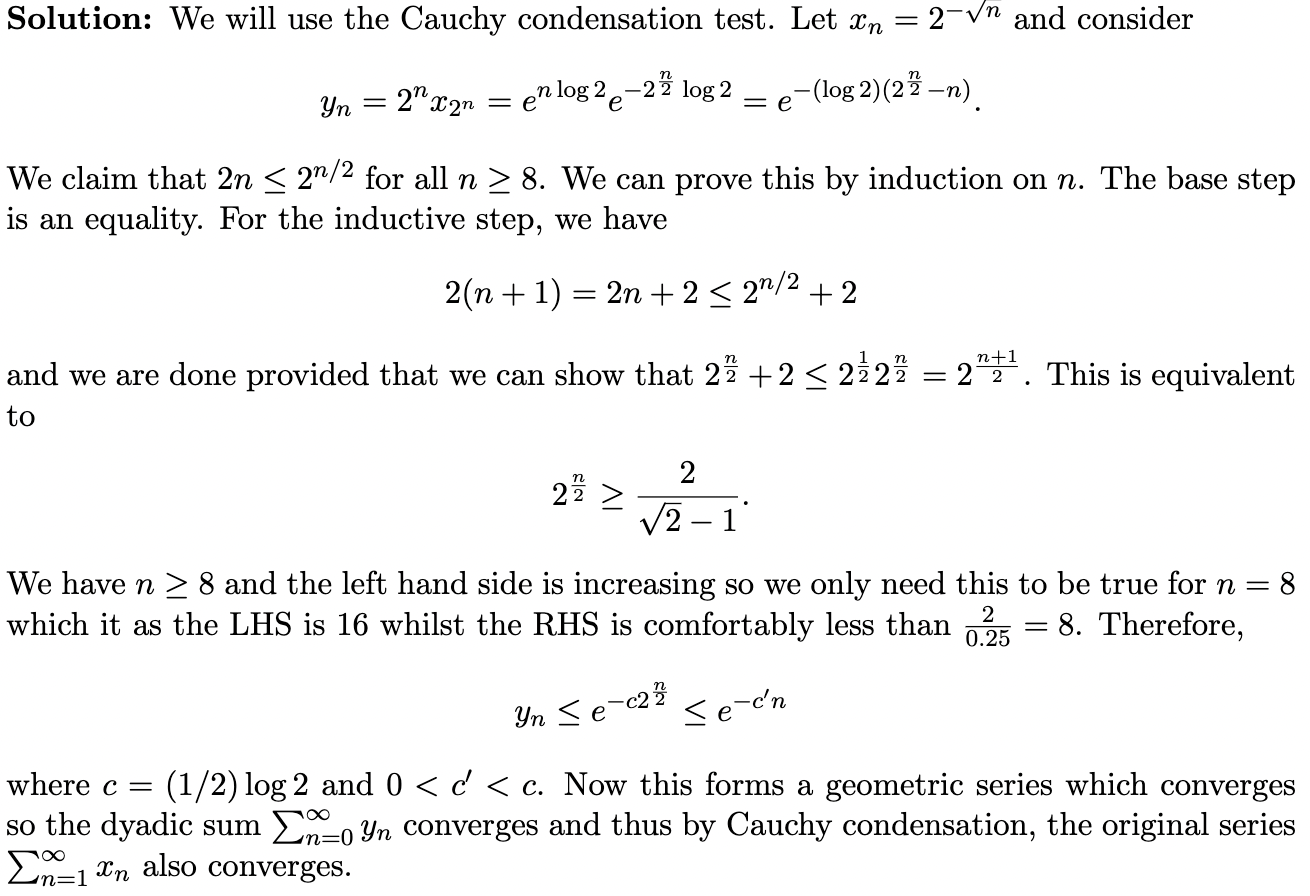
\includegraphics[scale = 0.5]{seq}  
\end{center}
\textbf{Let $A \subseteq \mathbb{R}$ s.t. there exists a sequence $(x_n) \in
A$ converging to a real number $x_0 \not\in A$. Show there exists an
unbounded continuous function on A.} \\
\textit{\textbf{Proof:}} Let $f : A \to \mathbb{R}$ be given by $f(x)
= \frac{1}{x - x_0}$. Since $x_0 \not\in A$, $f(x)$ is well-defined on
all of $A$. It is clearly continuous by the ALT. We show it is
unbounded. Let $M > 0$ be given and choose $\varepsilon =
\frac{1}{M}$. Since $x_n \to x_0$, there exists $N \in \mathbb{N}$
s.t. $|x_n - x_0| < \varepsilon$. So $\left| f(x) \right| =
\frac{1}{\left| x_n - x_0 \right|} > M$. \\ \\
\textbf{Prove $\lim \frac{n + 6}{n^2 - 6} = 0$}
\begin{align*}
  \bigg| \frac{n + 6}{n^2 - 6} - 0 \bigg| &< \varepsilon \\
  \bigg| \frac{n + 6}{n^2 - 6} \bigg| &< \varepsilon
\end{align*}
Note that when $n \geq 6$, we have that $|n + 6| \leq 2n$, $|n^2 - 6|
\geq \frac{1}{2}n^2$.
\begin{align*}
  \bigg| \frac{n + 6}{n^2 - 6} \bigg| \leq \frac{2n}{\frac{1}{2}n^2}
  &< \varepsilon \\
  \frac{4n}{n^2} < \varepsilon \\
  \frac{4}{n} < \varepsilon \\
  n > \max{\{\frac{4}{\varepsilon}, 6\}}
\end{align*}
Let $\varepsilon > 0$. Let $N \geq \max{\{\frac{4}{\varepsilon}, 6\}}$. Then
$\forall n > N$, we have
\[n > \max{\{\frac{4}{\varepsilon}, 6\}} \implies \bigg| \frac{n + 6}{n^2 - 6}
  \bigg| \leq \frac{2n}{\frac{1}{2}n^2} < \varepsilon\]
\end{document}

%%% Local Variables:
%%% mode: latex
%%% TeX-master: t
%%% End:
